\documentclass[12pt, a4paper, twoside]{article}
\usepackage[utf8]{inputenc}
\usepackage[cm]{fullpage}
\usepackage{fancyhdr}
\usepackage{textcomp}
\usepackage{graphicx}

\begin{document}

\title{Relatório do Experimento 3 de OAC}
\author{
Arthur Bizzi: 13/0102636 \\
Arthur da Silveira Couto: 16/0002575 \\
Caio Albuquerque Brandão: 16/0003636 \\
Cristiano Silva Júnior: 13/0070629 \\
Leonardo Maffei: 16/0033811 \\}
\date{7 de Junho de 2017}
\maketitle

\section{Exercício 1}

A fim de comparar as simulações do MARS e de forma de onda, compilamos o programa \textit{testePIPE.s} no MARS e rodamos em ambas plataformas.

No MARS, o programa, ao ser executado, não fez nada. Contudo, ao se comentar as linhas de hazard de controle, o programa é capaz de terminar a sua execução.

Ao simular em forma de onda, o programa gerou a forma de onda na figura 1.

% Como adicionar uma figura
\begin{figure}
    \centering
    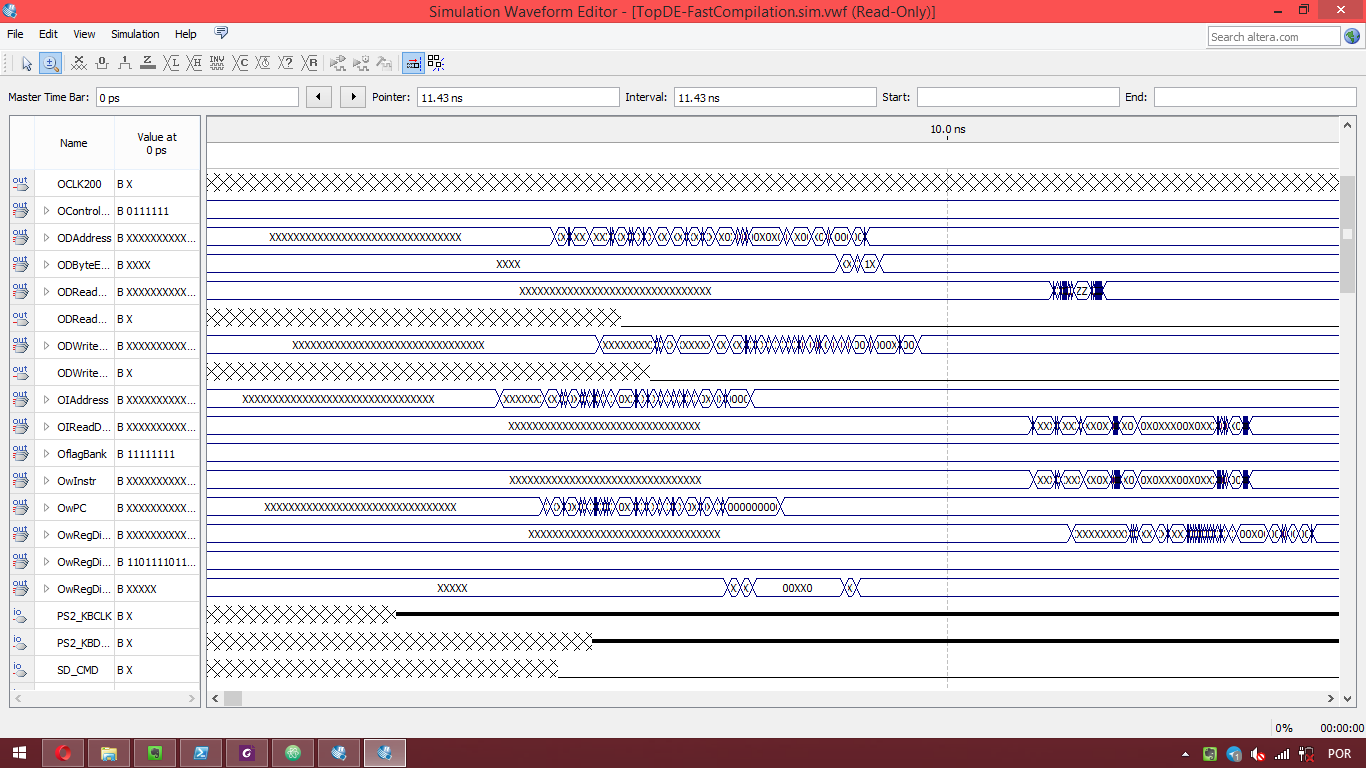
\includegraphics[width=0.8\textwidth]{./figs/sim1.png}
    \caption{Simulação em forma de onda.}
\end{figure}

\section{Exercício 2}

% TODO Diagrama de blocos do caminho de dados
% TODO Tabela verdade da unidade de controle

\section{Exercício 3}

% TODO Analisar unidades de Hazard e Forward

\section{Exercício 4}

% TODO Simular forma de onda do programa teste.s

\section{Exercício 5}

% TODO Linkar vídeos de desenho das bandeiras

\section{Exercício 6}

% TODO Incluir bolhas para realizar operações de ponto flutuante

\section{Exercício 7}

% TODO Comparar síntese da FPULA

\section{Exercício 8}

% TODO Implementar ceil
% TODO Implementar floor
% TODO Implementar round

\end{document}
